\documentclass[sigconf,nonacm]{acmart}

\begin{document}

\title{COS 487 / 587 Course Project Part 1: IR Rangers}

\author{Esther Greene}
\affiliation{%
  \institution{University of Southern Maine}
  \city{Portland}
  \state{Maine}
  \country{USA}}
\email{esther.greene@maine.edu}

\author{Courtney Jackson}
\affiliation{%
  \institution{University of Southern Maine}
  \city{Portland}
  \state{Maine}
  \country{USA}}
\email{courtney.jackson@maine.edu}

\author{Nathaniel Serrano}
\affiliation{%
  \institution{University of Southern Maine}
  \city{Portland}
  \state{Maine}
  \country{USA}}
\email{nathaniel.serrano@maine.edu}

\begin{abstract}
  ...
\end{abstract}

\keywords{information retrieval, ...}

\maketitle

\section{Introduction}
The volume of scientific literature makes finding relevant work
increasingly difficult, both at the level of whole papers and of the
specific passages that answer a question. This paper describes the first
phase of our retrieval system for arXiv papers, which applies two
traditional term-matching models, TF-IDF and BM25, to retrieving both
papers and individual paragraphs. We describe our preprocessing of a
noisy collection, tune BM25 per task, evaluate both models with
significance testing, and analyze where term matching succeeds and where
it fails, particularly on hard queries that paraphrase technical
terminology. As we will detail, our findings show that BM25 
significantly outperforms TF-IDF on both tasks.

The test collection consists of 34,308 arXiv papers published in August
and September 2024. Each paper is provided both as raw HTML scraped from
the ar5iv website and as a processed JSON file containing its identifier,
title, abstract, and paragraphs. Because the JSON files were produced with
rule-based extraction, they contain noise such as leftover \LaTeX{} markup
and merged words, which we discuss in Section~\ref{sec:preprocessing}.
In total, the collection contains 2,275,574 paragraphs, or about 66 paragraphs 
per paper.

We address two tasks over this collection: \emph{paper retrieval}, which
returns papers identified by their arXiv ID (in YYMM.NNNNN format), and
\emph{paragraph retrieval}, which returns individual paragraphs. For each
query, systems return their top 100 results. Three query sets are
provided: Train (2,000 queries), Study (250 queries with relevance
judgments, which we use for all analysis in this paper), and Test (250
queries whose judgments are withheld). Each set contains 30\% easy, 50\%
medium, and 20\% hard queries. Relevance is graded on a three-point
scale: a document that fully addresses the query is relevant (2), one that
provides useful information without fully addressing it is partially
relevant (1), and any document not in the judgments is considered
non-relevant.

\section{Methodology}
\label{sec:method}

Our system processes both retrieval tasks with a single pipeline.
Documents and queries are first cleaned and tokenized
(Section~\ref{sec:preprocessing}); the processed text is used to build
two collections, one of papers and one of paragraphs
(Section~\ref{sec:docrep}), each with its own inverted index. Two ranking
models, TF-IDF (Section~\ref{sec:tfidf}) and BM25
(Section~\ref{sec:bm25}), score documents from these indexes; both use
identical preprocessing and the same indexes, so differences between them
reflect only their scoring functions. Section~\ref{sec:eval} describes our
evaluation setup, and Section~\ref{sec:interface} the search interface.

Throughout, $N$ denotes the number of documents in a collection,
$\mathit{df}_t$ the number of documents containing term $t$,
$\mathit{tf}_{t,d}$ the number of occurrences of $t$ in document $d$,
and $L_d$ and $L_{\mathit{avg}}$ the length of $d$ and the average
document length, in tokens.
\subsection{Preprocessing}
\label{sec:preprocessing}

Documents and queries pass through the same preprocessing pipeline, so
that query terms match the terms stored in the index. All settings are
read from a YAML configuration file, and a copy of the configuration is
saved with the processed collections; queries are tokenized with that
saved copy at search time. The final pipeline applies the following
steps in order:

\begin{enumerate}
  \item \textbf{Text cleaning.} Inline mathematics delimited by dollar
    signs, remaining \LaTeX{} commands (e.g., \texttt{\textbackslash mathcal}),
    URLs, and numeric citation markers such as ``[5, 6, 7]'' are each
    replaced with a space.
  \item \textbf{Lowercasing.}
  \item \textbf{Tokenization.} Text is split into runs of letters and
    digits. Underscores act as separators, so a subscript such as
    \texttt{x\_i} yields \texttt{x} and \texttt{i}.
  \item \textbf{Token filtering.} Tokens shorter than two characters and
    tokens consisting only of digits are discarded.
  \item \textbf{Stopword removal.} Stopwords are frequent function words,
    such as ``the'' and ``and'', that say little about a document's topic.
    We use NLTK's English list~\cite{bird2009nltk}, extended with terms
    common in scientific writing: ``et'', ``al'', ``fig'', ``figure'',
    ``table'', ``eq'', and ``section''.
  \item \textbf{Stemming.} Remaining tokens are reduced to stems with the
    Snowball English stemmer~\cite{porter2001snowball}, so that forms
    such as ``model'' and ``models'' match.
\end{enumerate}

The cleaning and filtering steps were motivated by corpus statistics.
With only lowercasing and stopword removal, the 50 most frequent tokens
were dominated by mathematical notation rather than words: digits
(``1'', ``2'', ``0''), single-letter variables (``n'', ``x'', ``k''),
underscores from subscripts, and \LaTeX{} commands such as ``mathcal''
and ``mathbb''. Adding these to the stopword list would also remove real
words such as ``text'' and ``prime'', so we instead remove inline math as
a whole. A lone dollar sign, such as in a price, would be paired with a
math delimiter and the text between them deleted, so math spans are only
removed from paragraphs with an even number of dollar signs. Only 1,458
paragraphs (0.06\%) contain an unpaired dollar sign. They keep their math
spans, although \LaTeX{} command removal and the token filters still
remove most of the resulting tokens. We evaluate the effects of our choice
to employ inline math removal and stemming on retrieval in Section~\ref{sec:analysis}.

Some extraction noise is not addressed by preprocessing. Adjacent words
are occasionally merged (e.g., ``andenthusiasts'', ``inmedical''), and
this also occurs in queries: Test query 2251 contains ``sustainedvowel''.
Such tokens cannot match their component words. Display equations are
absent from the extracted text altogether, and the \texttt{abstract}
field contains more merged words than the copy of the abstract that
appears as each paper's first paragraph (Section~\ref{sec:docrep}).

\begin{table}[h]
  \caption{Paragraph collection statistics under three preprocessing
    settings, defined in Section~\ref{sec:preprocessing}.}
  \label{tab:cleaning}
  \small
  \begin{tabular}{lrrr}
    \toprule
    & Baseline & Cleaned & + Snowball \\
    \midrule
    Total tokens           & 167,965,275 & 114,907,087 & 114,907,087 \\
    Unique terms           & 781,405     & 659,861     & 589,251 \\
    Terms appearing once   & 367,415     & 297,672     & 272,983 \\
    Median length          & 58          & 40          & 40 \\
    90th pct.\ length      & 143         & 104         & 104 \\
    Longest paragraph      & 32,070      & 20,818      & 20,818 \\
    Over 1,000 tokens      & 868         & 117         & 117 \\
    Empty paragraphs       & 429         & 8,389       & 8,389 \\
    Under 10 tokens        & 82,390      & 230,782     & 230,782 \\
    \bottomrule
  \end{tabular}
\end{table}
Table~\ref{tab:cleaning} compares three settings. \emph{Baseline}
applies only lowercasing, tokenization on letters, digits, and
underscores, and stopword removal (with ``not'' and ``no'' retained).
\emph{Cleaned} applies steps 1--5 and no longer retains ``not'' and
``no'': bag-of-words models cannot use them to express negation, and
``not'' alone accounted for over 500,000 tokens. \emph{+ Snowball} is the final
pipeline. Cleaning reduced the collection from 168.0 million to 114.9
million tokens, a 31.6\% decrease, and all of the 50 most frequent tokens
became words, such as ``model'', ``data'', and ``using''. It also reduced
the number of paragraphs longer than 1,000 tokens from 868 to 117; the
longest Baseline paragraphs were collaboration author lists made up
largely of \LaTeX{} markup and ORCID identifiers. Stemming leaves the
number of tokens unchanged but shrinks the vocabulary by a further
10.7\%, from 659,861 to 589,251 terms. The cost is that some distinct
words share a stem: ``different'' and ``difference'' both become
``differ'', and ``generate'', ``generation'', and ``generative'' all
become ``generat''. Table~\ref{tab:cleaning} also shows that the number
of paragraphs under 10 tokens nearly triples (82,390 $\rightarrow$ 230,782). 
This is because the cleaning process employed in the latter two pipelines
strips math out of math-heavy paragraphs and leaves only their prose, causing
many to become short fragments. Finally, cleaning removes every token from 8,389 
paragraphs. Of these, 94\% contain inline math or \LaTeX{} commands: 
they are standalone formulas, sometimes with a few connecting words 
(``if'', ``then'', ``where'') that are themselves stopwords. We describe 
how these paragraphs are handled in Section~\ref{sec:docrep}.

\subsection{Document Representation}
\label{sec:docrep}
\subsection{TF-IDF}
\label{sec:tfidf}
\subsection{BM25}
\label{sec:bm25}
BM25 addresses two weaknesses of the TF-IDF weighting in
Section~\ref{sec:tfidf}: it saturates the contribution of repeated terms,
and it normalizes document length relative to the collection average
rather than by vector length. We describe the scoring function we use,
our implementation, and how we tuned its two parameters, $k_1$ and $b$,
for each collection.
\subsubsection{Scoring Function}

\begin{equation}
  \mathrm{score}(q,d) = \sum_{t \in q} \mathit{idf}_t \cdot
    \frac{\mathit{tf}_{t,d}\,(k_1 + 1)}
         {\mathit{tf}_{t,d} + k_1 \bigl(1 - b + b\,L_d / L_{\mathit{avg}}\bigr)}
  \label{eq:bm25}
\end{equation}
\begin{equation}
  \mathit{idf}_t = \ln\!\left(1 + \frac{N - \mathit{df}_t + 0.5}{\mathit{df}_t + 0.5}\right)
  \label{eq:idf}
\end{equation}

\subsubsection{Implementation}
\subsubsection{Parameter Tuning}
% \begin{figure}[h]
%   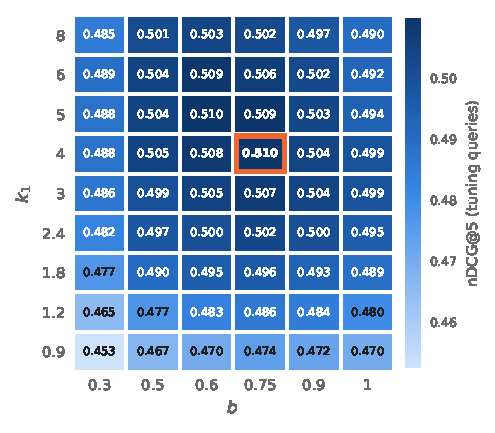
\includegraphics[width=\columnwidth]{figures/bm25_tuning_paper_full.pdf}
% \caption{BM25 nDCG@5 scores on 1,600 training queries (paper collection). 
% Rows represent $k_1$ values and columns represent $b$ values (not to scale); 
% all scores are rounded to three decimal places. The outlined cell marks the 
% selected setting ($k_1 = 4.0, b = 0.75$), which achieved the highest score 
% prior to rounding. This optimal setting lies within a broad plateau 
% ($k_1 \geq 3, 0.5 \leq b \leq 0.9$) where scores differ by roughly 
% 0.01 or less, meaning neighboring parameters (e.g., $k_1 = 5, b = 0.6$) 
% perform equivalently.}
%   \label{fig:tuning-paper}
% \end{figure}

% \begin{figure}[h]
%   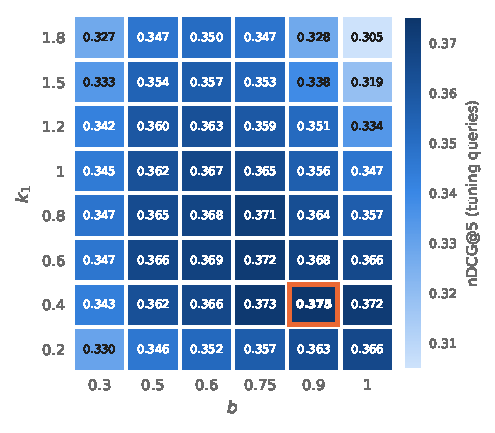
\includegraphics[width=\columnwidth]{figures/bm25_tuning_paragraph_full.pdf}
% \caption{Paragraph tuning results}
%   \label{fig:tuning-paragraph}
% \end{figure}

\subsection{Evaluation Setup}
\label{sec:eval}

\subsection{Search Interface}
\label{sec:interface}

\section{Evaluation Results}
\subsection{Metrics}
\subsection{Efficiency}

\section{Results Analysis}
\label{sec:analysis}

\begin{table}[h]
  \caption{Preprocessing ablation on Study queries, nDCG@5, with BM25
    parameters fixed to the values tuned for the main configuration
    (math removed, Snowball stemming). Comparing the first two columns
    isolates math removal; comparing the last two isolates stemming.
    $^{*}$ marks a significant difference from the column to its left
    (paired t-test, $p < 0.05$).}
  \label{tab:ablation}
  \small
  \begin{tabular}{lrrr}
    \toprule
    & Main & Math kept & Math kept, \\
    &      &           & no stemming \\
    \midrule
    Papers, TF-IDF     & 0.313 & 0.320 & 0.379$^{*}$ \\
    Papers, BM25       & 0.514 & 0.534$^{*}$ & 0.542 \\
    Paragraphs, TF-IDF & 0.229 & 0.238 & 0.235 \\
    Paragraphs, BM25   & 0.416 & 0.416 & 0.378$^{*}$ \\
    \bottomrule
  \end{tabular}
\end{table}

We isolated two preprocessing choices on Study queries
(Table~\ref{tab:ablation}). Removing inline math, which reduced the
collection by 31.6\%, had little effect on retrieval. It made no
significant difference for either model on paragraphs or for TF-IDF on
papers, and slightly reduced paper BM25 (nDCG@5 0.534 to 0.514,
significant only for nDCG@5 and strict P@5). Papers contain enough
spelled-out notation, such as ``epsilon'' or ``kappa'', for kept math
tokens to provide a few additional correct matches. Math removal is a 
reasonable tradeoff for a 31.6\% reduction in collection size.

Stemming mattered more, in opposite directions for our two strongest
effects. It significantly improved paragraph BM25 on every metric
(nDCG@5 0.378 to 0.416, MRR 0.457 to 0.509), but significantly reduced
paper TF-IDF on every metric (nDCG@5 0.379 to 0.320); it had no
significant effect on paper BM25 or paragraph TF-IDF. A plausible
explanation is that short paragraphs gain from the additional matches
stemming creates, while for long papers under cosine normalization,
conflated stems (e.g., ``generat'' for ``generate'', ``generation'', and
``generative'') make common stems even more frequent and dilute term
weights. Regardless, it is important to note that even TF-IDF's best 
configuration (no stemming, 0.379 nDCG@5) stays far below BM25 (0.542).
This implies that the reasons for BM25's better performance over TF-IDF
do not necessarily originate from the preprocessing pipeline.
\section{Conclusion}

\bibliographystyle{ACM-Reference-Format}
\bibliography{references}

\end{document}